\documentclass[12pt]{article}
\usepackage[a3paper,landscape]{geometry}
% \usepackage[a0paper,landscape]{geometry}
\usepackage[poster]{tcolorbox}
\usepackage{pagecolor}
\usepackage{background}
\usepackage{mdframed}
\pagestyle{empty}
\pagecolor{red}
% \usepackage[dvipsnames]{xcolor}
\begin{document}
\begin{tcbposter}[
coverage = {spread,
% interior style={top color=yellow,bottom color=yellow!50!red}
interior style={top color=cyan,bottom color=cyan!50!red}
% interior style={\color{OliveGreen}}
% interior style={top color = blue}
},
% poster = {showframe,columns=3,rows=2},
poster = {columns=3,rows=2},
% boxes = {fonttitle = \bfseries\Large\scshape}
boxes = {fonttitle = \bfseries\Large\scshape},
fontsize = 16pt
]
% Here, we insert the poster content later
\posterbox{name=title,column=2,span=2,above=bottom}{
    %\resizebox{18cm}{!}{\bfseries\Huge My Important Project}\\[3mm]
    %Hans.Mustermann@deepthought.university
    \underline{David Amaro-Alcala}, Barry C. Sanders, Hubert de Guise
}
\posterbox[adjusted title = Summary, colframe = teal!50!black, colback=teal!50]{
    % name=project,column=1, above=bottom
    column = 1,
    name=project, 
    between=top and bottom
}{
    % \Large
% \textbf{Characterising} gates is necessary to decide if a quantum computer (the gates) implementation scales.
% A particularly interesting set of gates is a generator of \textbf{universal gates}, like H and T.
{\Huge We characterise a set of generators of universal qutrit gates, via the \textbf{average gate fidelity}.}
% We introduce a group that includes a \textbf{qutrit} T gate.
% Show that the standard \textbf{Randomised Benchmarking} protocol can be extended to estimate the average gate fidelity of the T gate.
%David Amaro Alcala

\includegraphics[width=\textwidth]{auxiliary figures/crazy-scientist.pdf}
}

\posterbox[adjusted title = Characterise]{
    % name=project,column=1, above=bottom
    name=result, 
% between = title and top,
    column = 2,row =1
% sequence = 1 between title and top then 2 between title and process}{}
    % column=2,
    % above=title
    % between=top and bottom
    % column=2,span=1
}{
% Characterise means showing that the gates from a quantum computer work 
% ---within a certain error threshold---as expected.    
% The characterisation is done by extending the 
% dihedral benchmarking technique from qubits to qutrits.
% {\LARGE
{
% original
% Randomised Benchmarking schemes names a family of methods used to characterise quantum gates.
% The characterisation, in Randomised Benchmarking schemes, is done via the average gate fidelity.
% This fidelity is estimated by randomly sampling gates from the relevant gate set, and experimentally 
% estimating the fidelity of a sequence of gates that, if the gates were ideal, its composition would be 
% equal to the identity operation.
% summarized
Randomised Benchmarking is a method used to assess the quality of quantum gates
by estimating the average fidelity of a randomly selected set of gates from a
particular set. The fidelity is determined by comparing the behaviour of the
gates to the expected behaviour of ideal gates that would make up the identity
operation.
% RB methods characterise a gate set by estimating the average gate fidelity over such gate set.
% Here, we extend the dihedral benchmarking technique from qubits to
% qutrits; that is, we characterise a set of generators of a universal
% gate set.
}
% \tcblower

% \vfill

\includegraphics[width=\textwidth]{auxiliary figures/crazy-scientist.pdf}
}
% \end{tcolorbox}

% \posterbox[adjusted title = T gate, standard jigsaw, opacityback = 0]{
\posterbox[adjusted title = T gate]{
    % name=project,column=1, above=bottom
    name=result1, 
% between = title and top,
    column = 3,row =1
% sequence = 1 between title and top then 2 between title and process}{}
    % column=2,
    % above=title
    % between=top and bottom
    % column=2,span=1
}{
% original
% Randomised Benchmarking is commonly used to characterise Clifford
% gates. However, in order to outperform a classical computer, a quantum
% computer, in addition to the Clifford gate set, needs to implement a gate known as the T gate. However, by
% definition, the T gate is not a member of the Clifford
% group. Therefore, an extension RB to characterise T gates is
% needed. 
Randomised Benchmarking (RB) is commonly used to characterise Clifford gates,
but in order for a quantum computer to surpass a classical computer, it must
also be able to implement a T gate in addition to the Clifford gate set. T gates
are not part of the Clifford group, so an extension of RB is required to
characterize T gates.


\begin{center}
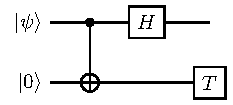
\includegraphics[width=0.5\textwidth]{auxiliary figures/universal-circuit.pdf}
\end{center}

A \textbf{qutrit} is a three-level system; that is, a system with two excited states.
Qutrits offer advantages with respect to qubits.
Moreover, qutrits nowadays are widely implemented, for example, in ion traps.
}

\posterbox[adjusted title = The HDG]{
    % name=project,column=1, above=bottom
    name=result2, 
% between = title and top,
column = 2,
between = result1 and title,
    % column = 2,row =2
% sequence = 1 between title and top then 2 between title and process}{}
    % column=2,
    % above=title
    % between=top and bottom
    % column=2,span=1
}{
% To obtain a simple expression, the operations to benchmark 
% need to form a group.
% We introduced the HyperDihedral group which is the 
% smallest group that includes the T gate and requires minimal post-processing data analysis.
Common Randomised Benchmarking schemes assume that the gates, being
characterised, correspond to the physical implementation of a group.
We were interested in the minimal (in order) group that included the T
gate. Such group, which we call HyperDihedral, is generated by the following three matrices:

\begin{center}
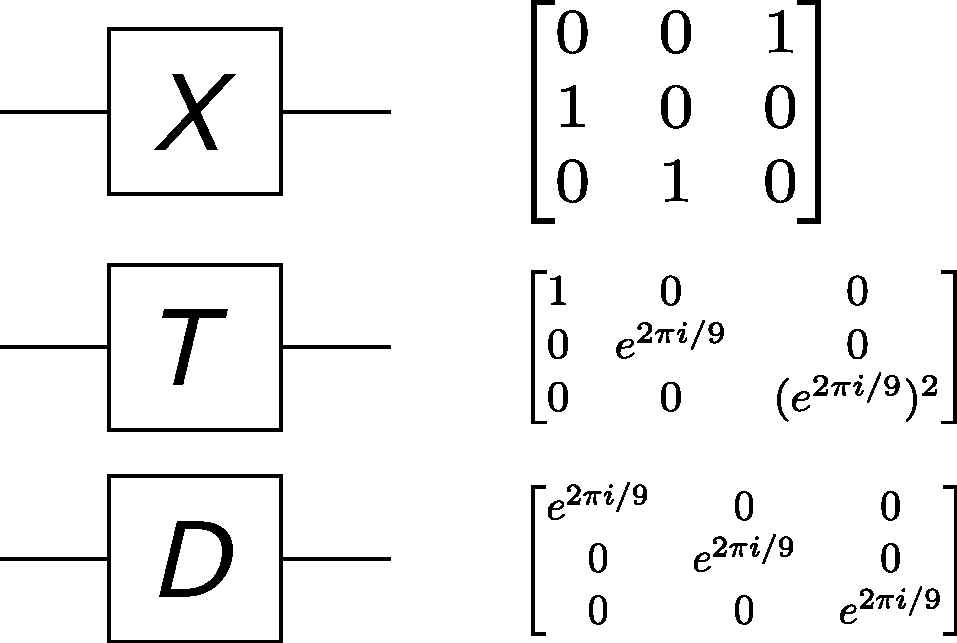
\includegraphics[width=0.7\textwidth]{auxiliary figures/matrices.pdf}
\end{center}
}

\posterbox[adjusted title = Results]{
    % name=project,column=1, above=bottom
    name=conclusion1, 
    column = 3,
% between = title and result,
between = result1 and title,
    % column = 3,row =2
% sequence = 1 between title and top then 2 between title and process}{}
    % column=2,
    % above=title
    % between=top and bottom
    % column=2,span=1
}{
We obtained an expression for the average gate fidelity over a HDG
implementation. Our formalism is valid under state preparation and
measurement imperfections and for gate-dependent errors. These two
conditions make our method part of the state-of-the-art in Randomised
Benchmarking schemes.


\begin{center}
\includegraphics[width=0.8\textwidth]{auxiliary figures/spplotandagf.pdf}
\end{center}
}

% \posterbox[adjusted title=Cover]{name =cover,
% sequence = 1 between title and bottom then 2 between title and process}{}
\end{tcbposter}
\end{document}